\documentclass[14pt]{extbook}
\usepackage{multicol, enumerate, enumitem, hyperref, color, soul, setspace, parskip, fancyhdr} %General Packages
\usepackage{amssymb, amsthm, amsmath, bbm, latexsym, units, mathtools} %Math Packages
\everymath{\displaystyle} %All math in Display Style
% Packages with additional options
\usepackage[headsep=0.5cm,headheight=12pt, left=1 in,right= 1 in,top= 1 in,bottom= 1 in]{geometry}
\usepackage[usenames,dvipsnames]{xcolor}
\usepackage{dashrule}  % Package to use the command below to create lines between items
\newcommand{\litem}[1]{\item#1\hspace*{-1cm}\rule{\textwidth}{0.4pt}}
\pagestyle{fancy}
\lhead{Progress Quiz 3}
\chead{}
\rhead{Version A}
\lfoot{}
\cfoot{}
\rfoot{Fall 2020}
\begin{document}

\begin{enumerate}
\litem{
Find the equation of the line described below. Write the linear equation as $ y=mx+b $ and choose the intervals that contain $m$ and $b$.\[ \text{Perpendicular to } 7 x - 8 y = 11 \text{ and passing through the point } (7, 3). \]\begin{enumerate}[label=\Alph*.]
\item \( m \in [0.98, 1.28] \hspace*{3mm} b \in [-6.3, -4.7] \)
\item \( m \in [-1.84, -1.11] \hspace*{3mm} b \in [-13.8, -10.2] \)
\item \( m \in [-1.84, -1.11] \hspace*{3mm} b \in [-4.4, -1.3] \)
\item \( m \in [-1.84, -1.11] \hspace*{3mm} b \in [9.6, 13.5] \)
\item \( m \in [-1.03, -0.51] \hspace*{3mm} b \in [9.6, 13.5] \)

\end{enumerate} }
\litem{
Solve the linear equation below. Then, choose the interval that contains the solution.\[ \frac{9x + 9}{4} - \frac{-8x -5}{7} = \frac{6x -4}{3} \]\begin{enumerate}[label=\Alph*.]
\item \( x \in [-3.17, -2.98] \)
\item \( x \in [-1.1, 0.16] \)
\item \( x \in [-2.2, -1.77] \)
\item \( x \in [-13.43, -11.97] \)
\item \( \text{There are no real solutions.} \)

\end{enumerate} }
\litem{
Write the equation of the line in the graph below in Standard form $Ax+By=C$. Then, choose the intervals that contain $A, B, \text{ and } C$.
\begin{center}
    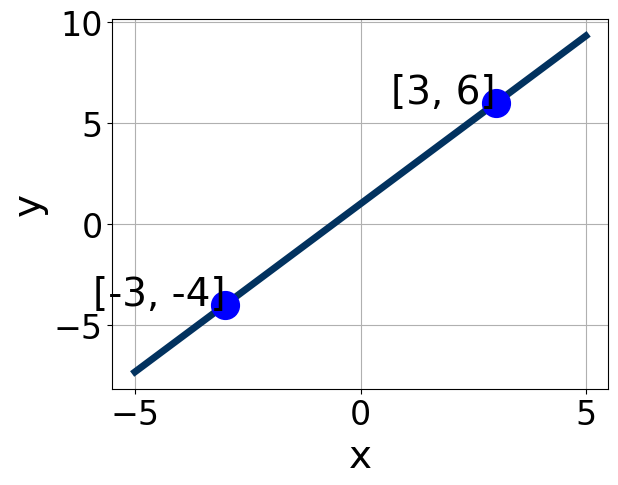
\includegraphics[width=0.5\textwidth]{../Figures/linearGraphToStandardA.png}
\end{center}
\begin{enumerate}[label=\Alph*.]
\item \( A \in [-6, -3], \hspace{3mm} B \in [1.47, 2.06], \text{ and } \hspace{3mm} C \in [-5, 6] \)
\item \( A \in [5, 8], \hspace{3mm} B \in [-2.44, -1.73], \text{ and } \hspace{3mm} C \in [-5, 6] \)
\item \( A \in [-2.5, 4.5], \hspace{3mm} B \in [-1.12, -0.95], \text{ and } \hspace{3mm} C \in [-5, 6] \)
\item \( A \in [5, 8], \hspace{3mm} B \in [1.47, 2.06], \text{ and } \hspace{3mm} C \in [-5, 6] \)
\item \( A \in [-2.5, 4.5], \hspace{3mm} B \in [0.71, 1.01], \text{ and } \hspace{3mm} C \in [-5, 6] \)

\end{enumerate} }
\litem{
Find the equation of the line described below. Write the linear equation as $ y=mx+b $ and choose the intervals that contain $m$ and $b$.\[ \text{Perpendicular to } 7 x - 9 y = 15 \text{ and passing through the point } (7, 9). \]\begin{enumerate}[label=\Alph*.]
\item \( m \in [-1.06, -0.3] \hspace*{3mm} b \in [15.3, 19.5] \)
\item \( m \in [0.72, 1.41] \hspace*{3mm} b \in [-3.2, 0.2] \)
\item \( m \in [-2.04, -1.28] \hspace*{3mm} b \in [0.7, 2.8] \)
\item \( m \in [-2.04, -1.28] \hspace*{3mm} b \in [15.3, 19.5] \)
\item \( m \in [-2.04, -1.28] \hspace*{3mm} b \in [-20.4, -17.7] \)

\end{enumerate} }
\litem{
First, find the equation of the line containing the two points below. Then, write the equation as $ y=mx+b $ and choose the intervals that contain $m$ and $b$.\[ (11, 2) \text{ and } (-2, -4) \]\begin{enumerate}[label=\Alph*.]
\item \( m \in [-0.46, 0.67] \hspace*{3mm} b \in [-3.38, -2.1] \)
\item \( m \in [-0.46, 0.67] \hspace*{3mm} b \in [-2.9, -1.79] \)
\item \( m \in [-0.46, 0.67] \hspace*{3mm} b \in [-9.49, -6.6] \)
\item \( m \in [-1.83, -0.29] \hspace*{3mm} b \in [-4.96, -4.42] \)
\item \( m \in [-0.46, 0.67] \hspace*{3mm} b \in [2.43, 3.33] \)

\end{enumerate} }
\litem{
Solve the linear equation below. Then, choose the interval that contains the solution.\[ \frac{5x -6}{7} - \frac{-9x -7}{4} = \frac{9x -5}{5} \]\begin{enumerate}[label=\Alph*.]
\item \( x \in [-6.9, -4.3] \)
\item \( x \in [0.4, 3.2] \)
\item \( x \in [-2.7, -1.1] \)
\item \( x \in [-1.5, 0] \)
\item \( \text{There are no real solutions.} \)

\end{enumerate} }
\litem{
Write the equation of the line in the graph below in Standard form $Ax+By=C$. Then, choose the intervals that contain $A, B, \text{ and } C$.
\begin{center}
    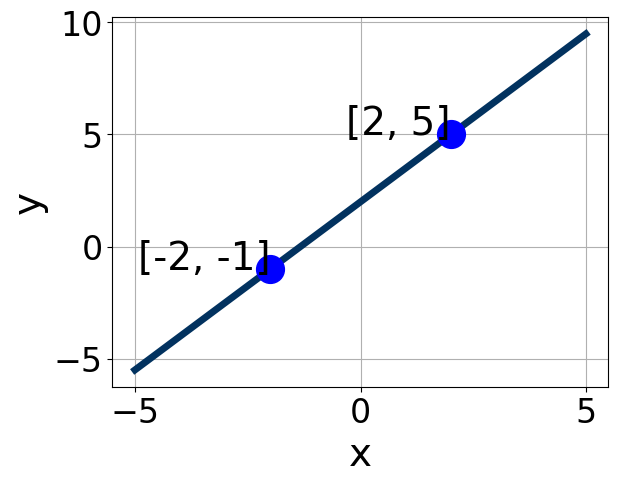
\includegraphics[width=0.5\textwidth]{../Figures/linearGraphToStandardCopyA.png}
\end{center}
\begin{enumerate}[label=\Alph*.]
\item \( A \in [-1.84, -0.56], \hspace{3mm} B \in [-1.38, -0.74], \text{ and } \hspace{3mm} C \in [-2.15, 0.06] \)
\item \( A \in [-4.07, -2.58], \hspace{3mm} B \in [1.37, 3.81], \text{ and } \hspace{3mm} C \in [3.93, 4.3] \)
\item \( A \in [2.43, 3.14], \hspace{3mm} B \in [-2.2, -1.35], \text{ and } \hspace{3mm} C \in [-4.71, -3.08] \)
\item \( A \in [2.43, 3.14], \hspace{3mm} B \in [1.37, 3.81], \text{ and } \hspace{3mm} C \in [3.93, 4.3] \)
\item \( A \in [-1.84, -0.56], \hspace{3mm} B \in [0.48, 1.93], \text{ and } \hspace{3mm} C \in [0, 3.52] \)

\end{enumerate} }
\litem{
Solve the equation below. Then, choose the interval that contains the solution.\[ -11(-2x -14) = -10(16x + 5) \]\begin{enumerate}[label=\Alph*.]
\item \( x \in [0.67, 1.15] \)
\item \( x \in [0.38, 0.74] \)
\item \( x \in [-0.6, -0.43] \)
\item \( x \in [-1.23, -0.98] \)
\item \( \text{There are no real solutions.} \)

\end{enumerate} }
\litem{
First, find the equation of the line containing the two points below. Then, write the equation as $ y=mx+b $ and choose the intervals that contain $m$ and $b$.\[ (4, -2) \text{ and } (-9, 7) \]\begin{enumerate}[label=\Alph*.]
\item \( m \in [-0.8, 0.3] \hspace*{3mm} b \in [-0.8, 0.3] \)
\item \( m \in [-0.8, 0.3] \hspace*{3mm} b \in [15.5, 16.9] \)
\item \( m \in [-0.8, 0.3] \hspace*{3mm} b \in [-7.9, -5.5] \)
\item \( m \in [-0.8, 0.3] \hspace*{3mm} b \in [-0.5, 2.2] \)
\item \( m \in [-0.4, 3.6] \hspace*{3mm} b \in [11.8, 13.4] \)

\end{enumerate} }
\litem{
Solve the equation below. Then, choose the interval that contains the solution.\[ -7(19x + 8) = -2(9x -13) \]\begin{enumerate}[label=\Alph*.]
\item \( x \in [-0.32, -0.22] \)
\item \( x \in [0.26, 0.27] \)
\item \( x \in [-0.87, -0.6] \)
\item \( x \in [-0.21, -0.15] \)
\item \( \text{There are no real solutions.} \)

\end{enumerate} }
\end{enumerate}

\end{document}